\documentclass[ngerman, parskip*]{scrartcl}
\usepackage[utf8]{inputenc} 
\usepackage[ngerman]{babel} % deutsche Sprache

\usepackage[decimalsymbol=comma,
            loctolang={DE:ngerman,UK:english},
            separate-uncertainty = true,
            multi-part-units=single
            ]{siunitx}
\usepackage{paralist}
\usepackage{amsmath}
\usepackage{graphicx}
\usepackage{booktabs}
\usepackage{float}
\usepackage{caption}
\usepackage{subcaption}
\usepackage{tabularx}
\usepackage{array}
\usepackage{commath}
\usepackage{amsfonts}


\title{Praktikum Klassische Physik Teil 2 (P2)}
\subtitle{Laser A}
\author{Simon Fromme, Philipp Laur}

\date{\today}

\begin{document}

\maketitle
\tableofcontents
\newpage

\section{Brewsterwinkel}

\subsection{Brechungsindex von Glas}

Der Bresterwinkel wird über die Reflexion des Laserstrahls an der Zimmerdecke beobachtet, für 
\begin{align*}
  \alpha_B &=  \SI{180}{\degree} - \SI{125}{\degree} \\
  &=  \SI{55}{\degree}
\end{align*} 
kann man hier ein Minimum der Intensität beobachten. Aus der bekannten Beziehung aus der Vorbereitung (Annahme für den Brechungsindex von Luft $n_{\textrm{Luft}} = 1$) ergibt sich der Brechungsindex des Glases zu
\begin{align*}
  n_{\textrm{Glas}} &= \tan(\alpha_B) \\
  &= 1,428.
\end{align*}

Dies liegt in der Größenordnung gängiger optischer Gläser.

Die Bestimmung des Brewsterwinkels über das Maximum der Transmission mithilfe eines Si-Photoelements ist ungenau, da das Spannungssignal des Photoelements während des Messvorgangs zu stark schwankt, um genau messen zu könne, wann das Maximum der Transmission erreicht ist.


\section{Beugung an Spalt, Steg, Kreisloch, Kreisblende und Kante}

\subsection{Bestimmung der Breite eines Spalts}

In diesem Versuchsteil wird die Breite eines Einfach-Spalts aus dem -nach Bestrahlung durch Laser-Licht erzeugtem- Beugungsmuster bestimmt. 

Hierzu wurde jeweils der Abstand des n-ten Beugungsminimums von der optischen Achse aus $y_n = \frac{1}{2}\cdot (y_n^{(l)} - y_n^{(r)})$ bestimmt, wobei $y_n^{(l)}$ die y-Position des links und $y_n^{(r)}$ die Position des rechts vom Hauptmaximum liegend Beugungsminimum n-ter Ordnung ist. Die ermittelten Werte für die ersten neun Beugungsminima sind in Tabelle \ref{table:2_1} dargestellt.

\begin{table}[!h]
\centering
\caption{Positionen der Beugungsminima}
\begin{tabular}{l|ccccccccc}
\toprule
$n$ & 1 & 2 & 3 & 4 & 5 & 6 & 7 & 8 & 9 \\ 
$y_n$ in $\si{\cm}$ & 0.60 & 1.15 & 1.75 & 2.30 & 2.80 & 3.40 & 3.85 & 4.35 & 4.95 \\ 
\bottomrule
\end{tabular}
\label{table:2_1}
\end{table}

Nun wird $y_n$ gegen $n$ aufgetragen und aus der Steigung der Regressionsgerade $m$ die Dicke des Haars zu $d = \frac{\lambda l}{m}$ bestimmt.

\begin{figure}
  \centering
  \caption{Regression zur Bestimmung von $m = \dfrac{\lambda \cdot l}{d}$ }
  % GNUPLOT: LaTeX picture with Postscript
\begingroup
  \makeatletter
  \providecommand\color[2][]{%
    \GenericError{(gnuplot) \space\space\space\@spaces}{%
      Package color not loaded in conjunction with
      terminal option `colourtext'%
    }{See the gnuplot documentation for explanation.%
    }{Either use 'blacktext' in gnuplot or load the package
      color.sty in LaTeX.}%
    \renewcommand\color[2][]{}%
  }%
  \providecommand\includegraphics[2][]{%
    \GenericError{(gnuplot) \space\space\space\@spaces}{%
      Package graphicx or graphics not loaded%
    }{See the gnuplot documentation for explanation.%
    }{The gnuplot epslatex terminal needs graphicx.sty or graphics.sty.}%
    \renewcommand\includegraphics[2][]{}%
  }%
  \providecommand\rotatebox[2]{#2}%
  \@ifundefined{ifGPcolor}{%
    \newif\ifGPcolor
    \GPcolortrue
  }{}%
  \@ifundefined{ifGPblacktext}{%
    \newif\ifGPblacktext
    \GPblacktexttrue
  }{}%
  % define a \g@addto@macro without @ in the name:
  \let\gplgaddtomacro\g@addto@macro
  % define empty templates for all commands taking text:
  \gdef\gplbacktext{}%
  \gdef\gplfronttext{}%
  \makeatother
  \ifGPblacktext
    % no textcolor at all
    \def\colorrgb#1{}%
    \def\colorgray#1{}%
  \else
    % gray or color?
    \ifGPcolor
      \def\colorrgb#1{\color[rgb]{#1}}%
      \def\colorgray#1{\color[gray]{#1}}%
      \expandafter\def\csname LTw\endcsname{\color{white}}%
      \expandafter\def\csname LTb\endcsname{\color{black}}%
      \expandafter\def\csname LTa\endcsname{\color{black}}%
      \expandafter\def\csname LT0\endcsname{\color[rgb]{1,0,0}}%
      \expandafter\def\csname LT1\endcsname{\color[rgb]{0,1,0}}%
      \expandafter\def\csname LT2\endcsname{\color[rgb]{0,0,1}}%
      \expandafter\def\csname LT3\endcsname{\color[rgb]{1,0,1}}%
      \expandafter\def\csname LT4\endcsname{\color[rgb]{0,1,1}}%
      \expandafter\def\csname LT5\endcsname{\color[rgb]{1,1,0}}%
      \expandafter\def\csname LT6\endcsname{\color[rgb]{0,0,0}}%
      \expandafter\def\csname LT7\endcsname{\color[rgb]{1,0.3,0}}%
      \expandafter\def\csname LT8\endcsname{\color[rgb]{0.5,0.5,0.5}}%
    \else
      % gray
      \def\colorrgb#1{\color{black}}%
      \def\colorgray#1{\color[gray]{#1}}%
      \expandafter\def\csname LTw\endcsname{\color{white}}%
      \expandafter\def\csname LTb\endcsname{\color{black}}%
      \expandafter\def\csname LTa\endcsname{\color{black}}%
      \expandafter\def\csname LT0\endcsname{\color{black}}%
      \expandafter\def\csname LT1\endcsname{\color{black}}%
      \expandafter\def\csname LT2\endcsname{\color{black}}%
      \expandafter\def\csname LT3\endcsname{\color{black}}%
      \expandafter\def\csname LT4\endcsname{\color{black}}%
      \expandafter\def\csname LT5\endcsname{\color{black}}%
      \expandafter\def\csname LT6\endcsname{\color{black}}%
      \expandafter\def\csname LT7\endcsname{\color{black}}%
      \expandafter\def\csname LT8\endcsname{\color{black}}%
    \fi
  \fi
  \setlength{\unitlength}{0.0500bp}%
  \begin{picture}(7200.00,5040.00)%
    \gplgaddtomacro\gplbacktext{%
      \csname LTb\endcsname%
      \put(682,704){\makebox(0,0)[r]{\strut{} 0}}%
      \put(682,1444){\makebox(0,0)[r]{\strut{} 1}}%
      \put(682,2184){\makebox(0,0)[r]{\strut{} 2}}%
      \put(682,2925){\makebox(0,0)[r]{\strut{} 3}}%
      \put(682,3665){\makebox(0,0)[r]{\strut{} 4}}%
      \put(682,4405){\makebox(0,0)[r]{\strut{} 5}}%
      \put(814,484){\makebox(0,0){\strut{} 0}}%
      \put(2012,484){\makebox(0,0){\strut{} 2}}%
      \put(3210,484){\makebox(0,0){\strut{} 4}}%
      \put(4407,484){\makebox(0,0){\strut{} 6}}%
      \put(5605,484){\makebox(0,0){\strut{} 8}}%
      \put(6803,484){\makebox(0,0){\strut{} 10}}%
      \put(176,2739){\rotatebox{-270}{\makebox(0,0){\strut{}$y_n$ in $\si{\cm}$}}}%
      \put(3808,154){\makebox(0,0){\strut{}$n$}}%
    }%
    \gplgaddtomacro\gplfronttext{%
      \csname LTb\endcsname%
      \put(5649,964){\makebox(0,0)[r]{\strut{}Regressionsgerade}}%
    }%
    \gplbacktext
    \put(0,0){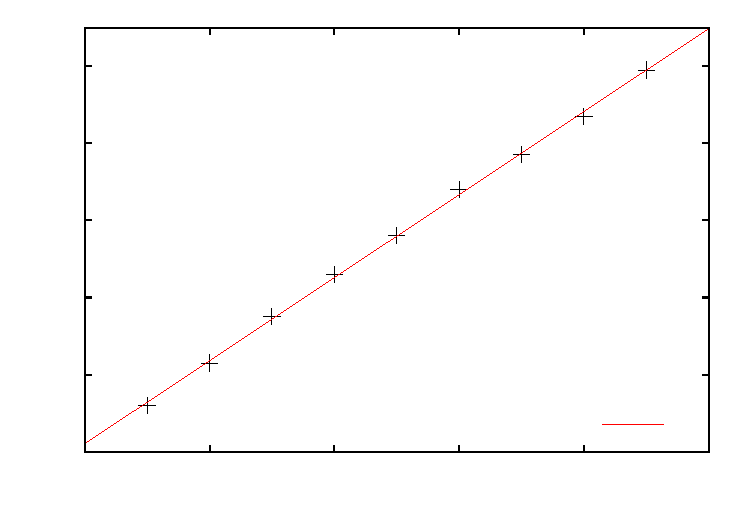
\includegraphics{Diagramme/2_1}}%
    \gplfronttext
  \end{picture}%
\endgroup

\end{figure}

Es ergibt sich 
\begin{align*}
  m = \SI {0,538}{\cm}
\end{align*}
und mit der Wellenlänge des Lasers $\lambda = \SI{632,8}{\nano\meter}$ und $l = \SI{289,8}{\cm} - \SI{59,3}{\cm} = \SI{230,5}{\cm}$ die Dicke des Spalts schließlich zu
\begin{align*}
  d = \SI{0,2709}{\milli\meter}.
\end{align*}
Dies entspricht in etwa dem angegebenen Spaltabstand von $ d = \SI{0,3}{\milli\meter}$.

Aus der Position des Spalts $x_1 = \SI{59,3}{\cm}$ und der Position des Schirms $x_2 = \SI{289,8}{\cm}$ ergibt sich der Abstand Spalt-Schirm zu $l = \SI{230,5}{\cm}$. Die Wellenlänge des Lasers war mit $\lambda = \SI{632,8}{\nano\meter}$ angegeben. 

\subsection{Vergleich der Beugungsfiguren von Spalt und Steg}

%% Hier fehlen die Bilder 

\subsection{Vergleich der Beugungsfiguren von Kreisöffnung, Kreisscheibe und Kante }

Im Versuch konnten die typischen (kreisförmigen) Beugungsminima bei der Beugung an Kreisöffnung und -scheibe nur sehr schlecht beobachet werden. Es konnten jedoch keine nennenswerten Unterschiede zwischen den beiden Beugungsbildern beobachtet werden, so dass man das Babinet-Theorem in diesem Fall bestätigen kann. 

%% Zuordnung der entsprechenden Beugungsbildern schwierig

\subsection{Durchmesser eines Haares aus Beugungsbild}

Nach dem Babinet-Theorem besitzt das Haar (Steg-förmig) das gleiche Beugungsbild, wie ein Spalt der selben Breite. Folglich kann die Haardicke analog zur ersten Teilaufgabe aus den Abständen der Beugungsminima bestimmt werden. Mit der bekannten Beziehung
\begin{align*}
  d = \dfrac{n\lambda l}{y_n} \Rightarrow y_n = \dfrac{\lambda \cdot l}{d}\cdot n
\end{align*}
bestimmt werden, wobei $y_n$ der Abstand des n-ten Beugungsminimums von der optischen Achse ist. 

Im Versuch wurde die Lage der Beugungsminima der Ordnung $n=1\dots 4$ vermessen. Die Messwerte sind in Tabelle \ref{table:2_4} dargestellt. 

\begin{table}[!h]
\centering
\caption{Positionen der Beugungsminima}
\begin{tabular}{l|cccc}
\toprule
$n$ & 1 & 2 & 3 & 4 \\ 
$y_n$ in $\si{\cm}$ & 1.90 & 3.75 & 5.65 & 7.45 \\ 
\bottomrule
\end{tabular}
\label{table:2_4}
\end{table}

Wie in 2.1 wird nun $y_n$ gegen $n$ aufgetragen und aus der Steigung der Regressionsgerade $m$ die Dicke des Haars zu $d = \frac{\lambda l}{m}$ bestimmt.

\begin{figure}
  \centering
  \caption{Regression zur Bestimmung von $m = \dfrac{\lambda \cdot l}{d}$ }
  % GNUPLOT: LaTeX picture with Postscript
\begingroup
  \makeatletter
  \providecommand\color[2][]{%
    \GenericError{(gnuplot) \space\space\space\@spaces}{%
      Package color not loaded in conjunction with
      terminal option `colourtext'%
    }{See the gnuplot documentation for explanation.%
    }{Either use 'blacktext' in gnuplot or load the package
      color.sty in LaTeX.}%
    \renewcommand\color[2][]{}%
  }%
  \providecommand\includegraphics[2][]{%
    \GenericError{(gnuplot) \space\space\space\@spaces}{%
      Package graphicx or graphics not loaded%
    }{See the gnuplot documentation for explanation.%
    }{The gnuplot epslatex terminal needs graphicx.sty or graphics.sty.}%
    \renewcommand\includegraphics[2][]{}%
  }%
  \providecommand\rotatebox[2]{#2}%
  \@ifundefined{ifGPcolor}{%
    \newif\ifGPcolor
    \GPcolortrue
  }{}%
  \@ifundefined{ifGPblacktext}{%
    \newif\ifGPblacktext
    \GPblacktexttrue
  }{}%
  % define a \g@addto@macro without @ in the name:
  \let\gplgaddtomacro\g@addto@macro
  % define empty templates for all commands taking text:
  \gdef\gplbacktext{}%
  \gdef\gplfronttext{}%
  \makeatother
  \ifGPblacktext
    % no textcolor at all
    \def\colorrgb#1{}%
    \def\colorgray#1{}%
  \else
    % gray or color?
    \ifGPcolor
      \def\colorrgb#1{\color[rgb]{#1}}%
      \def\colorgray#1{\color[gray]{#1}}%
      \expandafter\def\csname LTw\endcsname{\color{white}}%
      \expandafter\def\csname LTb\endcsname{\color{black}}%
      \expandafter\def\csname LTa\endcsname{\color{black}}%
      \expandafter\def\csname LT0\endcsname{\color[rgb]{1,0,0}}%
      \expandafter\def\csname LT1\endcsname{\color[rgb]{0,1,0}}%
      \expandafter\def\csname LT2\endcsname{\color[rgb]{0,0,1}}%
      \expandafter\def\csname LT3\endcsname{\color[rgb]{1,0,1}}%
      \expandafter\def\csname LT4\endcsname{\color[rgb]{0,1,1}}%
      \expandafter\def\csname LT5\endcsname{\color[rgb]{1,1,0}}%
      \expandafter\def\csname LT6\endcsname{\color[rgb]{0,0,0}}%
      \expandafter\def\csname LT7\endcsname{\color[rgb]{1,0.3,0}}%
      \expandafter\def\csname LT8\endcsname{\color[rgb]{0.5,0.5,0.5}}%
    \else
      % gray
      \def\colorrgb#1{\color{black}}%
      \def\colorgray#1{\color[gray]{#1}}%
      \expandafter\def\csname LTw\endcsname{\color{white}}%
      \expandafter\def\csname LTb\endcsname{\color{black}}%
      \expandafter\def\csname LTa\endcsname{\color{black}}%
      \expandafter\def\csname LT0\endcsname{\color{black}}%
      \expandafter\def\csname LT1\endcsname{\color{black}}%
      \expandafter\def\csname LT2\endcsname{\color{black}}%
      \expandafter\def\csname LT3\endcsname{\color{black}}%
      \expandafter\def\csname LT4\endcsname{\color{black}}%
      \expandafter\def\csname LT5\endcsname{\color{black}}%
      \expandafter\def\csname LT6\endcsname{\color{black}}%
      \expandafter\def\csname LT7\endcsname{\color{black}}%
      \expandafter\def\csname LT8\endcsname{\color{black}}%
    \fi
  \fi
  \setlength{\unitlength}{0.0500bp}%
  \begin{picture}(7200.00,5040.00)%
    \gplgaddtomacro\gplbacktext{%
      \csname LTb\endcsname%
      \put(682,704){\makebox(0,0)[r]{\strut{} 0}}%
      \put(682,1213){\makebox(0,0)[r]{\strut{} 1}}%
      \put(682,1722){\makebox(0,0)[r]{\strut{} 2}}%
      \put(682,2231){\makebox(0,0)[r]{\strut{} 3}}%
      \put(682,2740){\makebox(0,0)[r]{\strut{} 4}}%
      \put(682,3248){\makebox(0,0)[r]{\strut{} 5}}%
      \put(682,3757){\makebox(0,0)[r]{\strut{} 6}}%
      \put(682,4266){\makebox(0,0)[r]{\strut{} 7}}%
      \put(682,4775){\makebox(0,0)[r]{\strut{} 8}}%
      \put(814,484){\makebox(0,0){\strut{} 0}}%
      \put(2012,484){\makebox(0,0){\strut{} 1}}%
      \put(3210,484){\makebox(0,0){\strut{} 2}}%
      \put(4407,484){\makebox(0,0){\strut{} 3}}%
      \put(5605,484){\makebox(0,0){\strut{} 4}}%
      \put(6803,484){\makebox(0,0){\strut{} 5}}%
      \put(176,2739){\rotatebox{-270}{\makebox(0,0){\strut{}$y_n$ in $\si{\cm}$}}}%
      \put(3808,154){\makebox(0,0){\strut{}$n$}}%
    }%
    \gplgaddtomacro\gplfronttext{%
      \csname LTb\endcsname%
      \put(5649,1103){\makebox(0,0)[r]{\strut{}Regressionsgerade}}%
    }%
    \gplbacktext
    \put(0,0){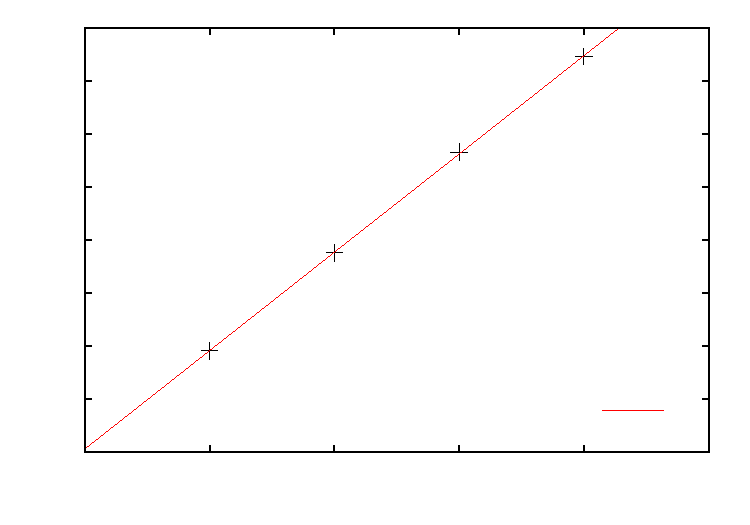
\includegraphics{Diagramme/2_4}}%
    \gplfronttext
  \end{picture}%
\endgroup

\end{figure}

Es ergibt sich 
\begin{align*}
  m = \SI {1,855}{\cm}
\end{align*}
und mit der Wellenlänge des Lasers $\lambda = \SI{632,8}{\nano\meter}$ und $l = \SI{289,8}{\cm} - \SI{56,2}{\cm} = \SI{233,6}{\cm}$ die Dicke des Haares schließlich zu
\begin{align*}
  d = \SI{79,69}{\micro\meter}.
\end{align*}
Mit der Micrometerschraube wurde eine Dicke von $d = \SI{55}{\micro\meter}$ bestimmt, was deutlich unter dem Wert aus dem Beugungsexperiment liegt. Dies kann dadurch erklärt werden, dass das Haar hier möglicherweise gequetscht wurde. 


%% Beginn: Aufgabenteil Philipp


\section{Beugung von Mehrfachspalten und Gittern}
\subsection{Ausmessung Doppelspalt}
Im Versuch wurde das Beugungsbild eines Doppelspalts (0,25/0,5) ausgemessen. Die Abstände der Minima werden der jeweiligen Ordung zugeordnet und die jeweilige Entfernung vom Haupmaximum gegen die jeweilige Ordnung aufgetragen. Durch diese Punkte wird analog zum bisherigen Vorgehen eine Ausgleichsgerade $f$ gelegt.
\begin{figure}
\centering
    
          \centering
          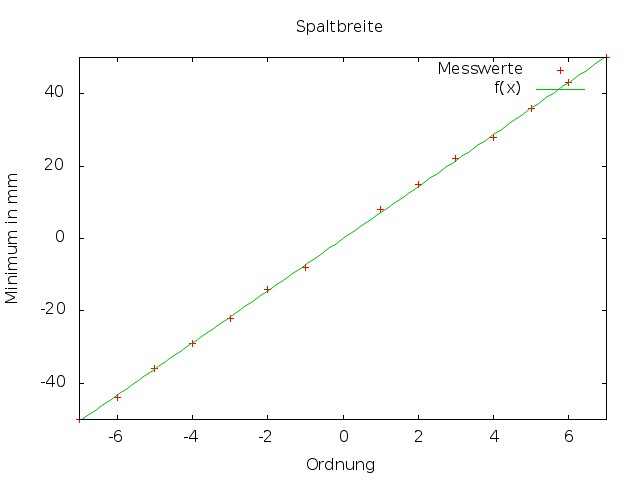
\includegraphics[width=\textwidth,natwidth=2560,natheight=1920]{Diagramme/doppel2.jpg}
          \caption{Doppelspalt, $d = \SI{0,25}{\mm}$, $b = \SI{0,50}{\milli\m}$}
\end{figure}

Es ergibt sich:
\begin{align*}
f(x)=7,2\cdot x-0,07143
\end{align*}
Mit der Beziehung aus der Vorbereitung für Beugungsminima am Doppelspalt
\begin{align*}
  y_n=\frac{\lambda l}{d}\cdot n\\
  l=\SI{2,455}{m},\ \lambda=\SI{632,8}{\nano\m}
\end{align*}
wird nun die Spaltbreite 
\begin{align*}
  d=\SI{0,216}{\milli\m}
\end{align*}
bestimmt.

Das Ergebniss liegt in der Nähe der Angabe, man konnte aber auch erkennen, dass der Doppelspalt schon leicht verbogen war. Außerdem ist die Abweichung durch eine nicht optimale Ausleuchtung und die schwierige Ablesbarkeit zu erklären.

Der Spaltabstand wurde wieder mittels einer linearen Regression bestimmt.
\begin{figure}
  \centering
  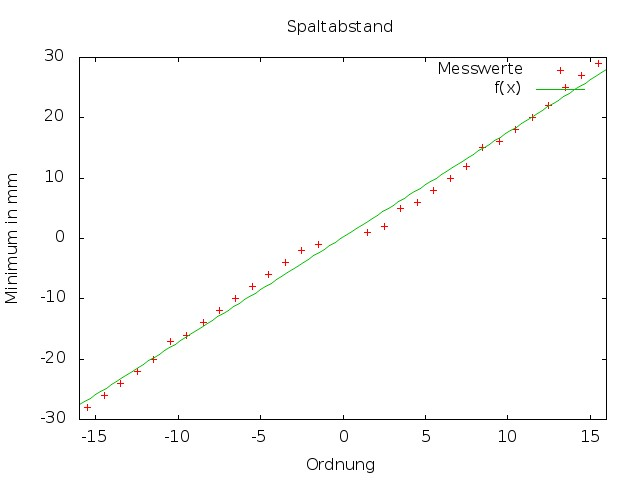
\includegraphics[width=\textwidth,natwidth=2560,natheight=1920]{Diagramme/doppel1.jpg}
  \caption{Doppelspalt, $d = \SI{0,25}{\mm}$, $b = \SI{0,50}{\mm}$}
\end{figure}
Die Ausgleichsgerade $g$ ergibt sich zu:
\begin{align*}
g(x)=1,73712\cdot x+0,2
\end{align*}
Aus der Auftragung
\begin{align*}
y_n=\frac{\lambda l}{d}\cdot (n+0,5)\\
l=2,365m,\ \lambda=\SI{632,8}{\nano\m}
\end{align*}
erhalten wir für den Spaltabstand 
\begin{align*}
d=\SI{0,862}{\milli\m}.
\end{align*}
Dieser weicht nun noch deutlicher von der Angabe ab und kann wiederum auf Ablesefehler zurückgeführt werden.
\subsection{Beugungsbilder von Doppel- und Dreifachspalt}
Der zweite Doppelspalt(0,25/0,75) hatte die gleiche Einhüllende aber einen größeren Abstand der Maximas, wie zu erwarten war.

\begin{figure}
\centering
        \begin{subfigure}[!h]{0.49\textwidth}
          \centering
          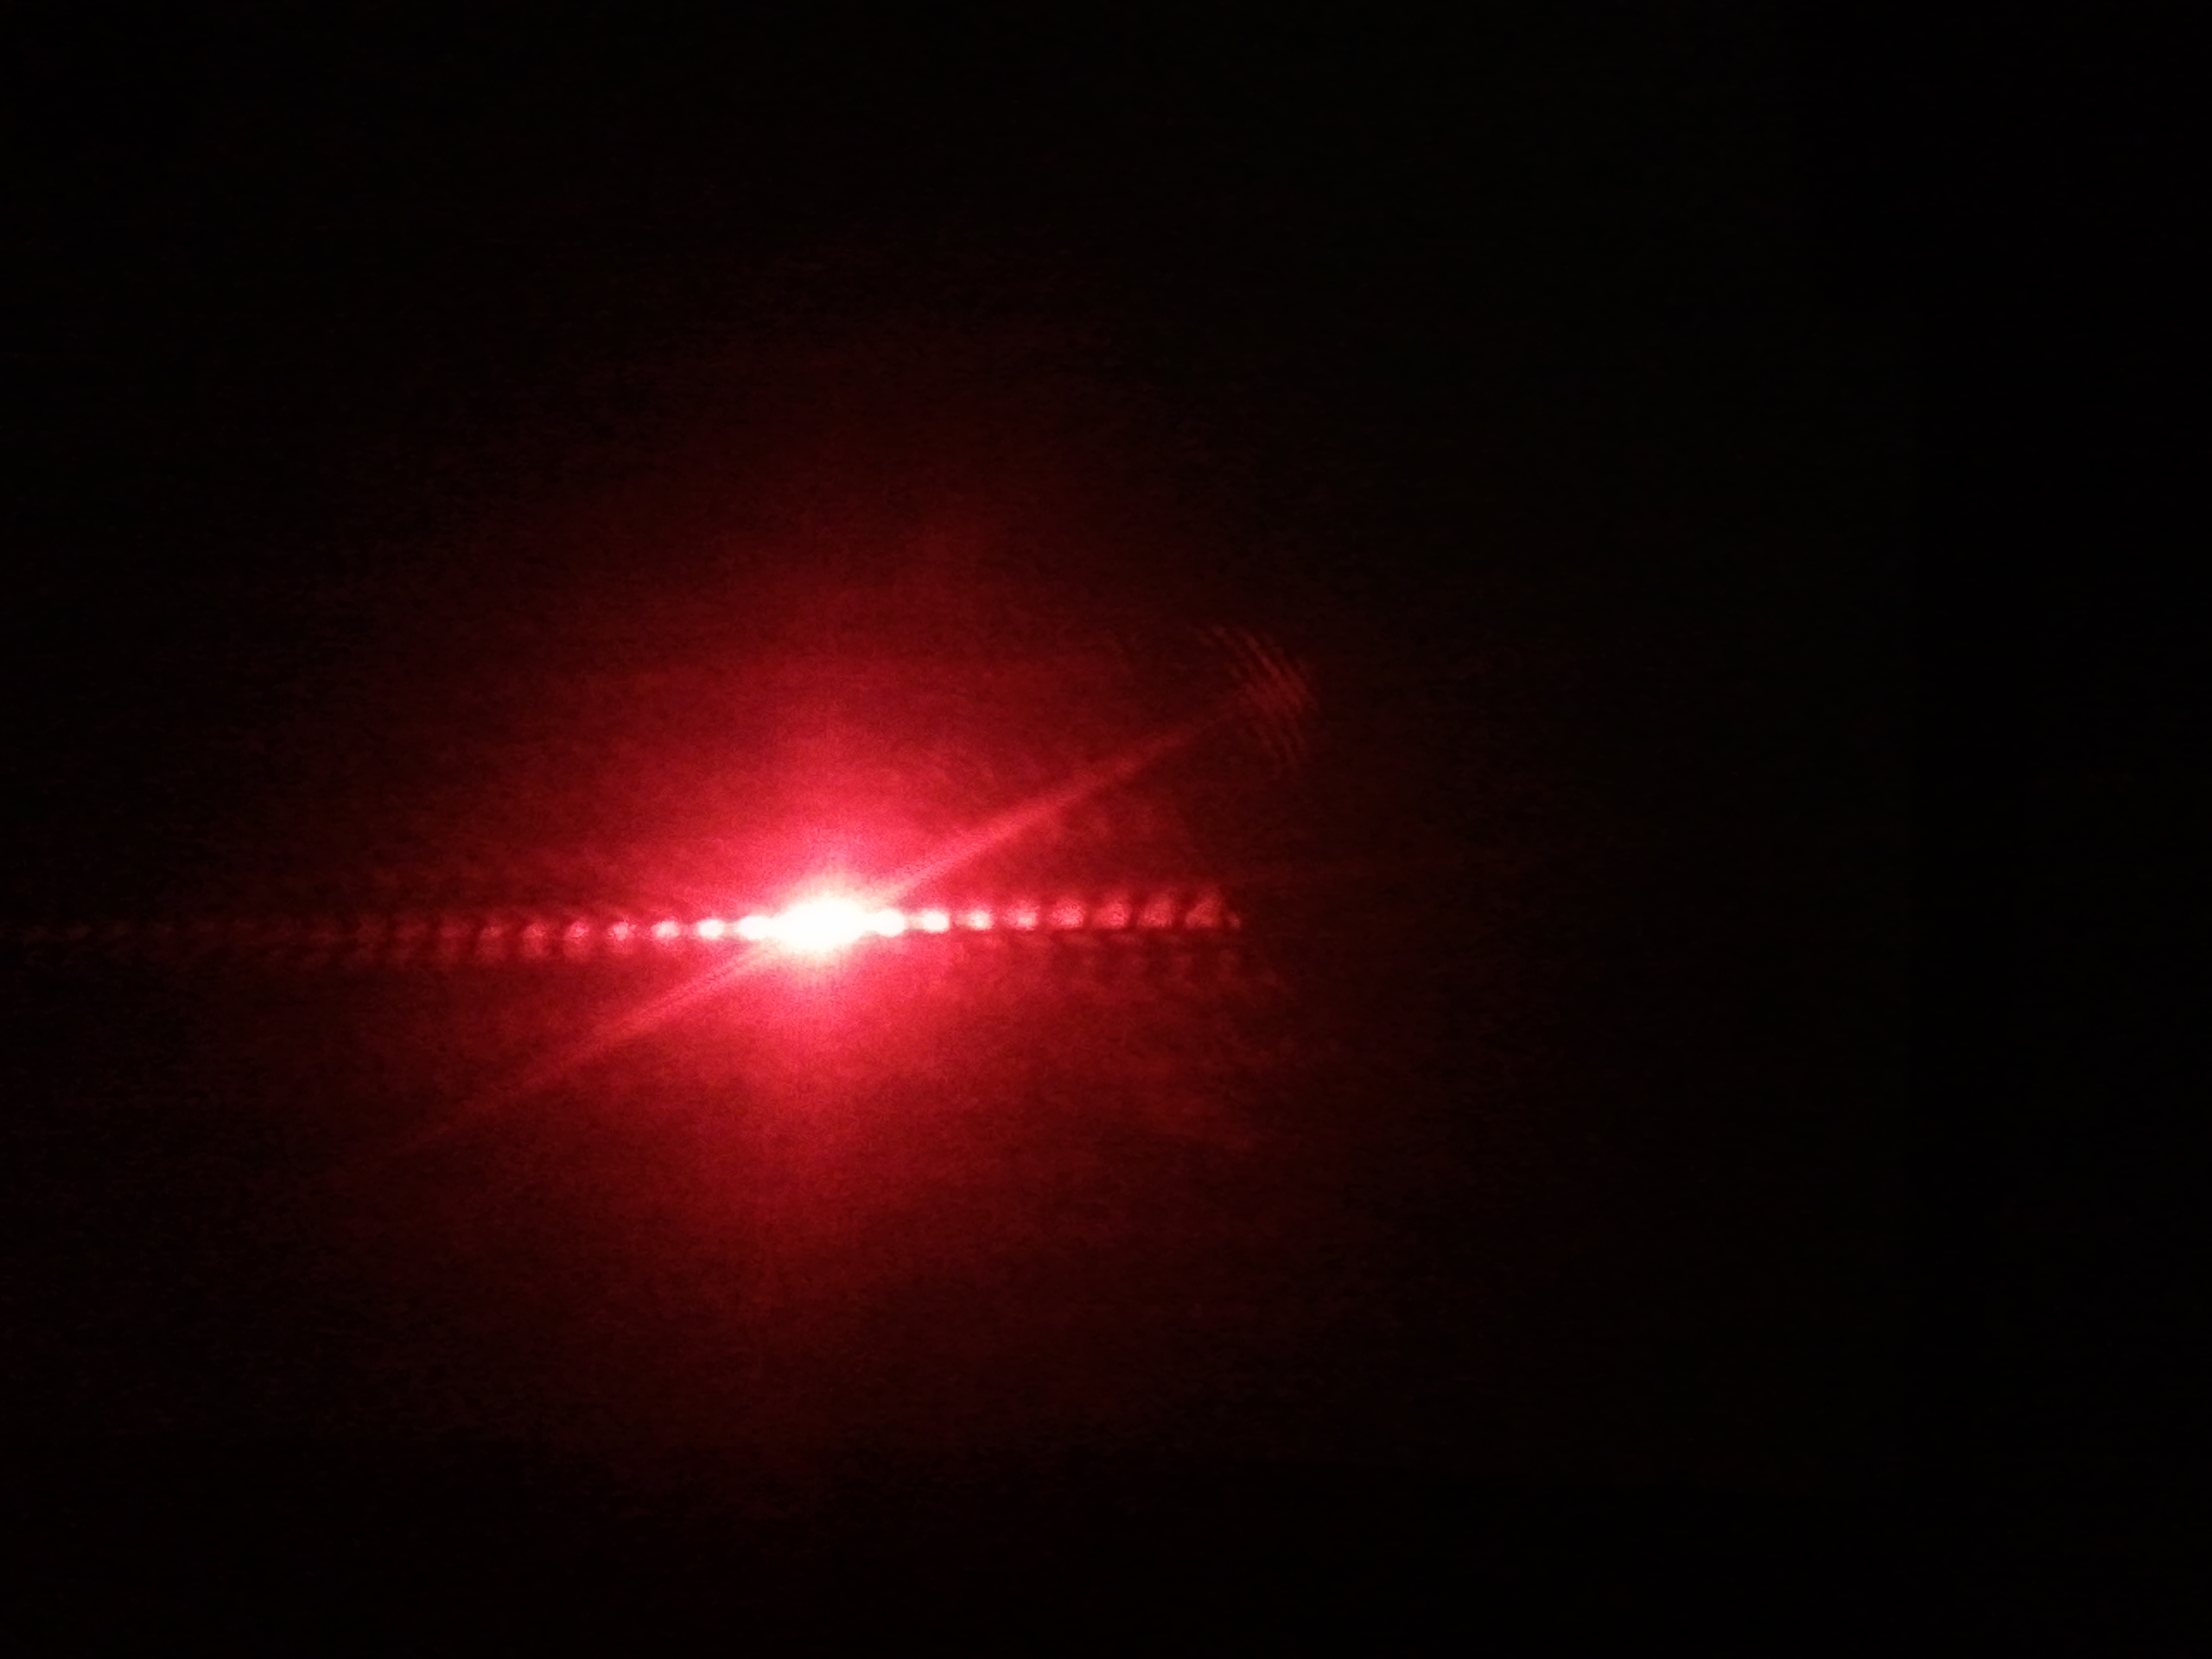
\includegraphics[width=\textwidth,natwidth=2560,natheight=1920]{Bilder/Doppelspalt_1.jpg}
          \caption{Doppelspalt, $d = \SI{0,25}{\mm}$, $b = \SI{0,50}{\mm}$}
        \end{subfigure}
        \begin{subfigure}[!h]{0.49\textwidth}
          \centering
          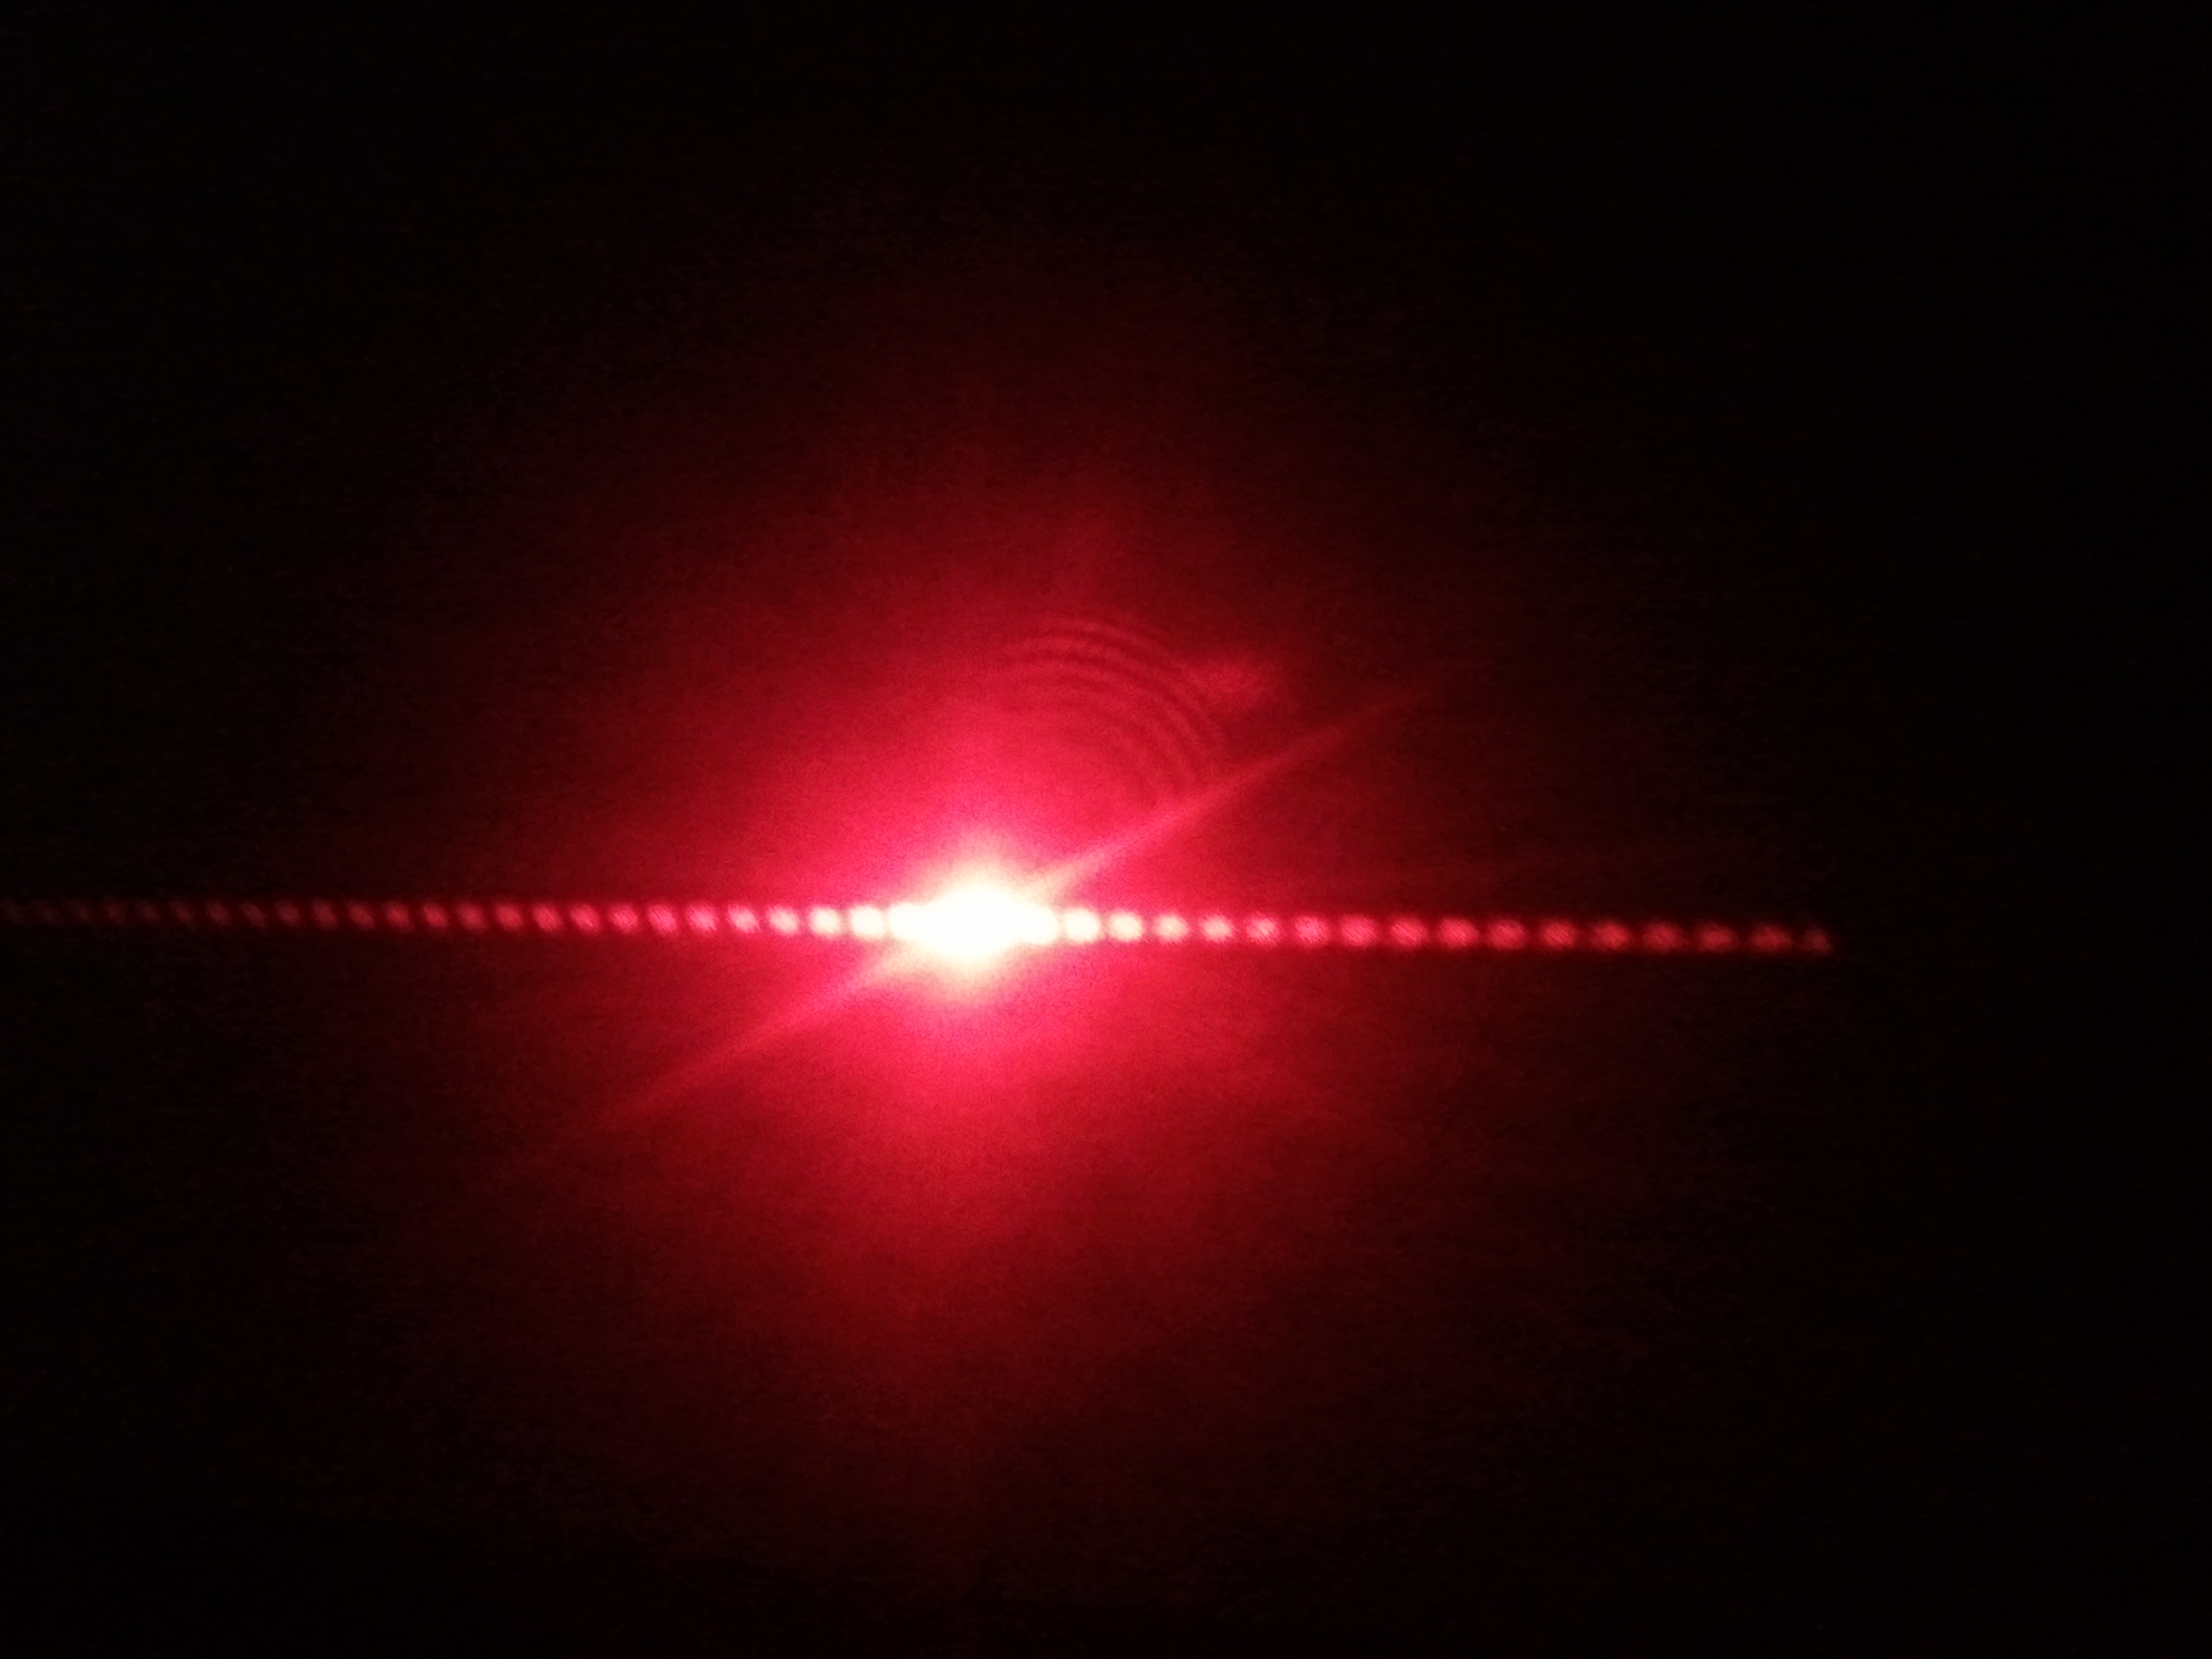
\includegraphics[width=\textwidth,natwidth=2560,natheight=1920]{Bilder/Doppelspalt_2.jpg}
          \caption{Doppelspalt, $d = \SI{0,25}{\mm}$, $b = \SI{0,75}{\mm}$}
        \end{subfigure}
\end{figure}

\begin{figure}
\centering
        \begin{subfigure}[!h]{0.49\textwidth}
          \centering
          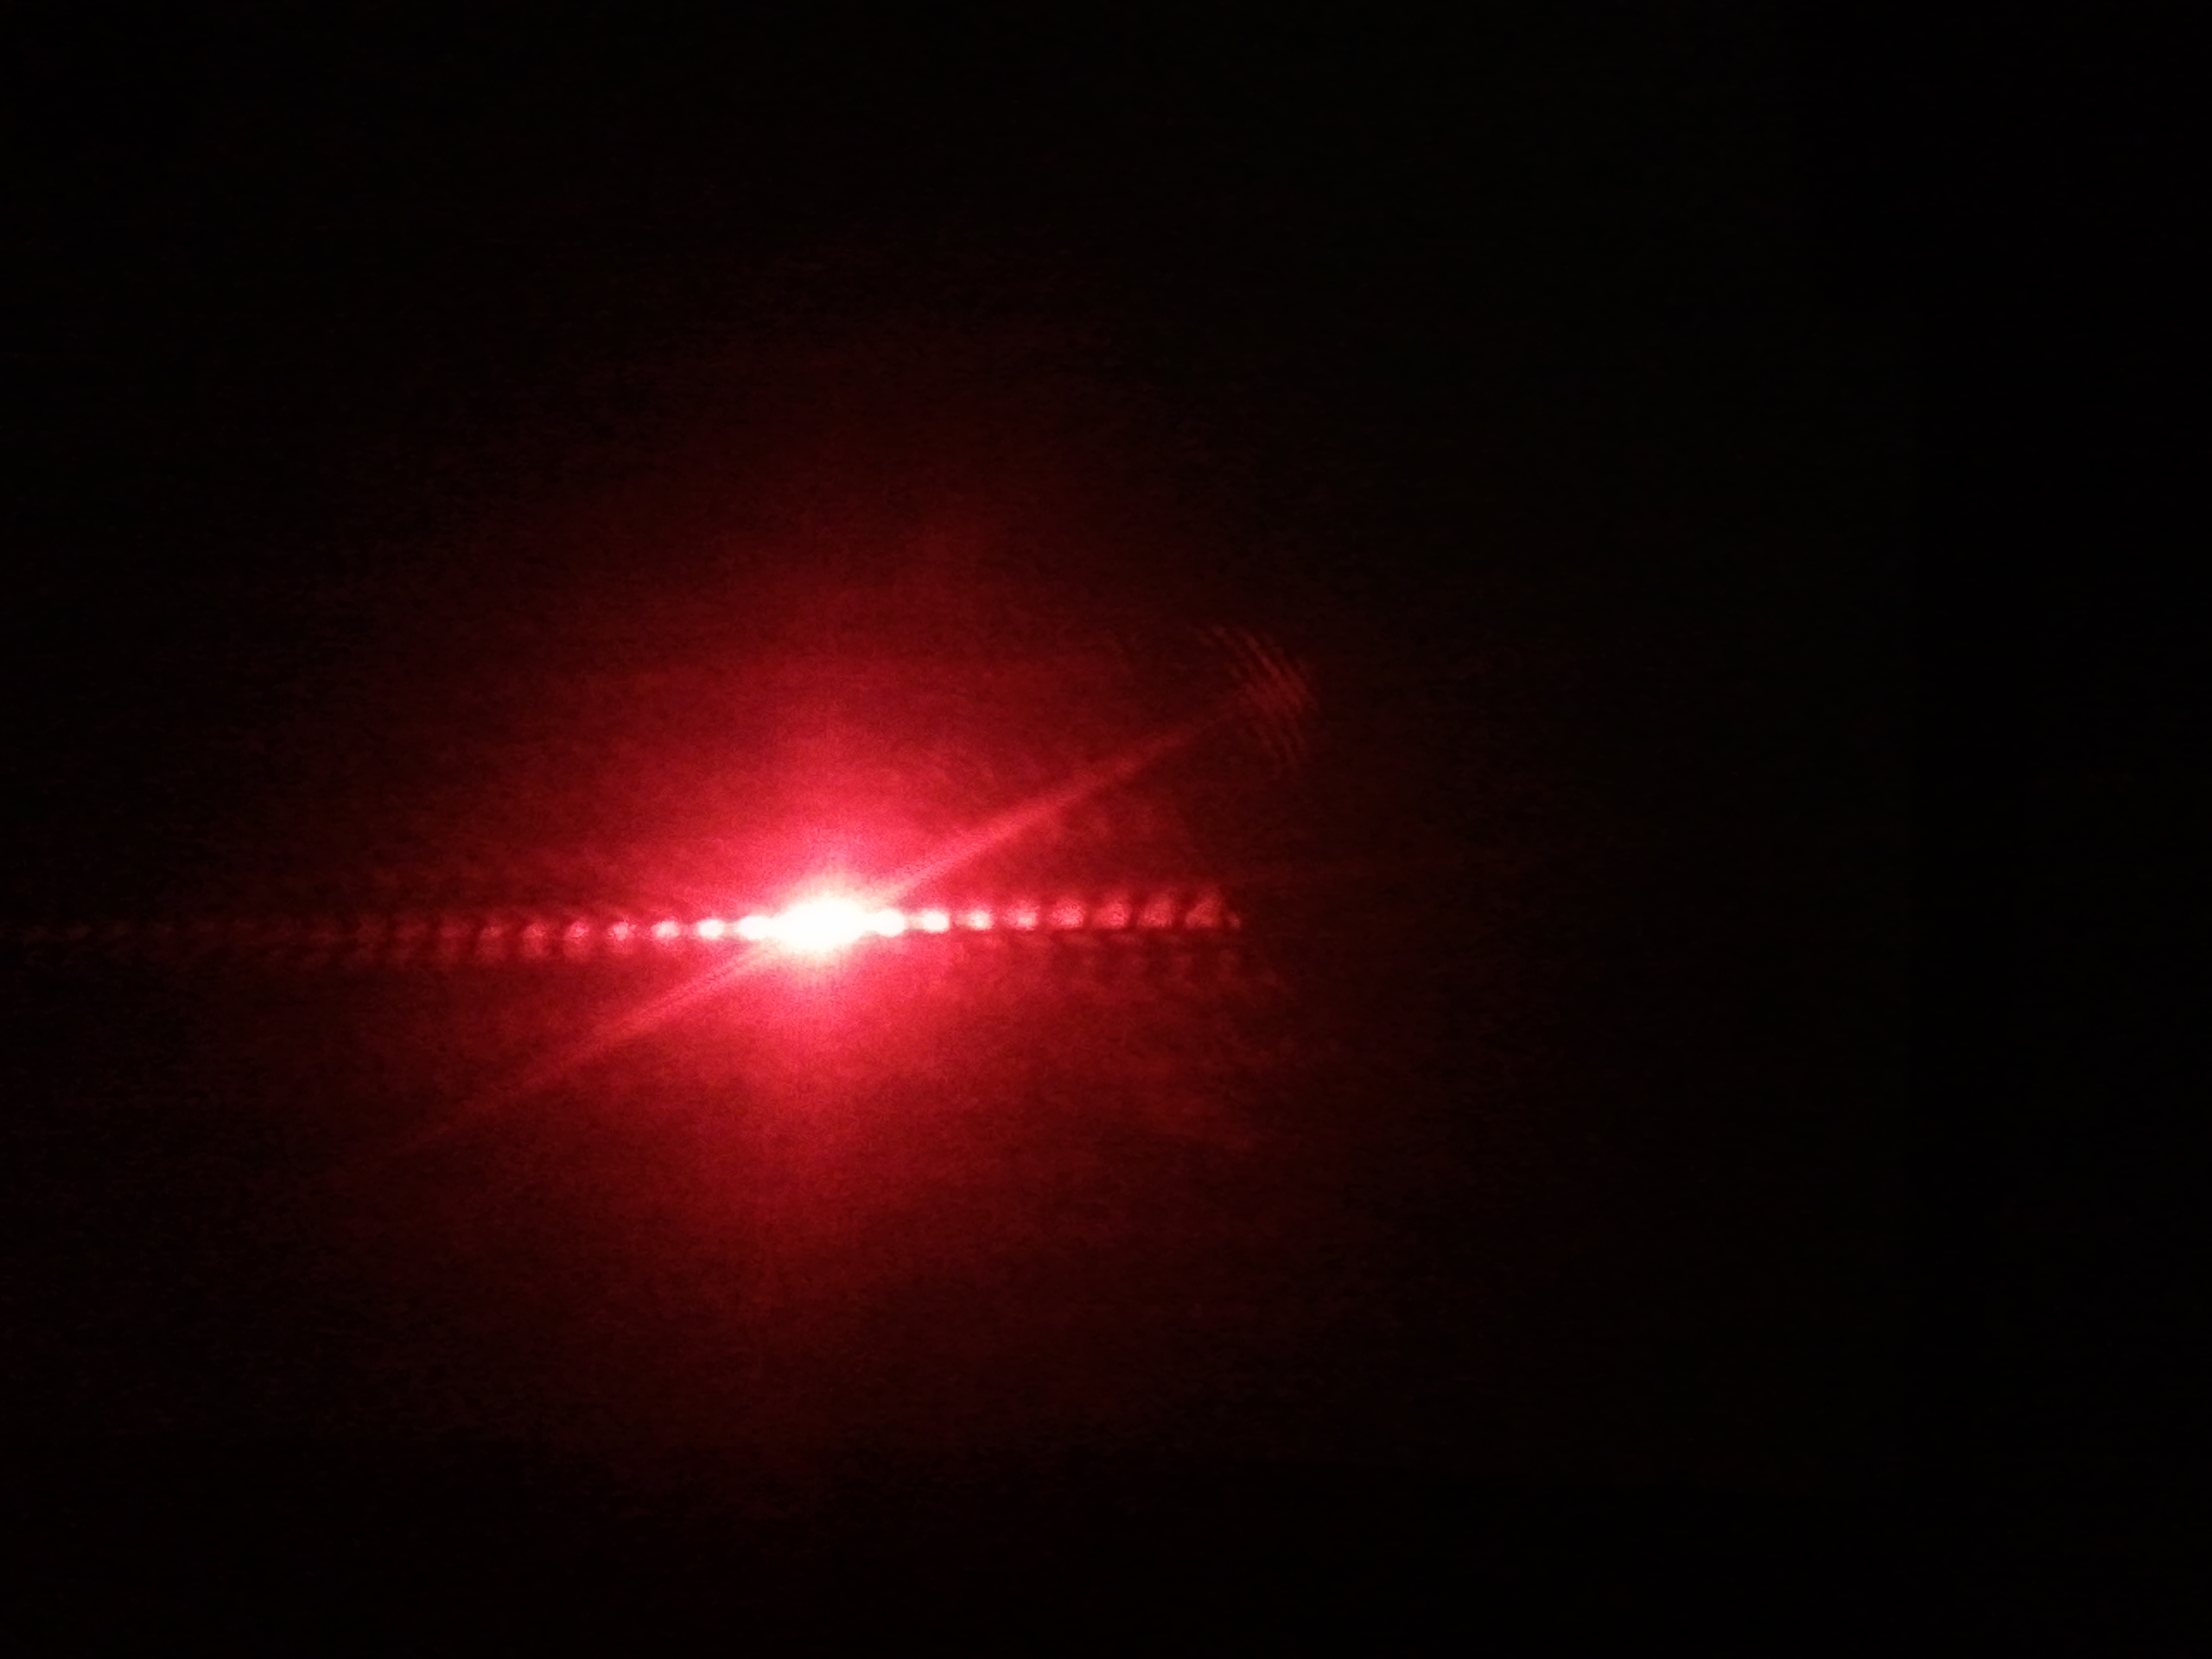
\includegraphics[width=\textwidth,natwidth=2560,natheight=1920]{Bilder/Doppelspalt_1.jpg}
          \caption{Doppelspalt, $d = \SI{0,25}{\mm}$, $b = \SI{0,50}{\mm}$}
        \end{subfigure}
        \begin{subfigure}[!h]{0.49\textwidth}
          \centering
          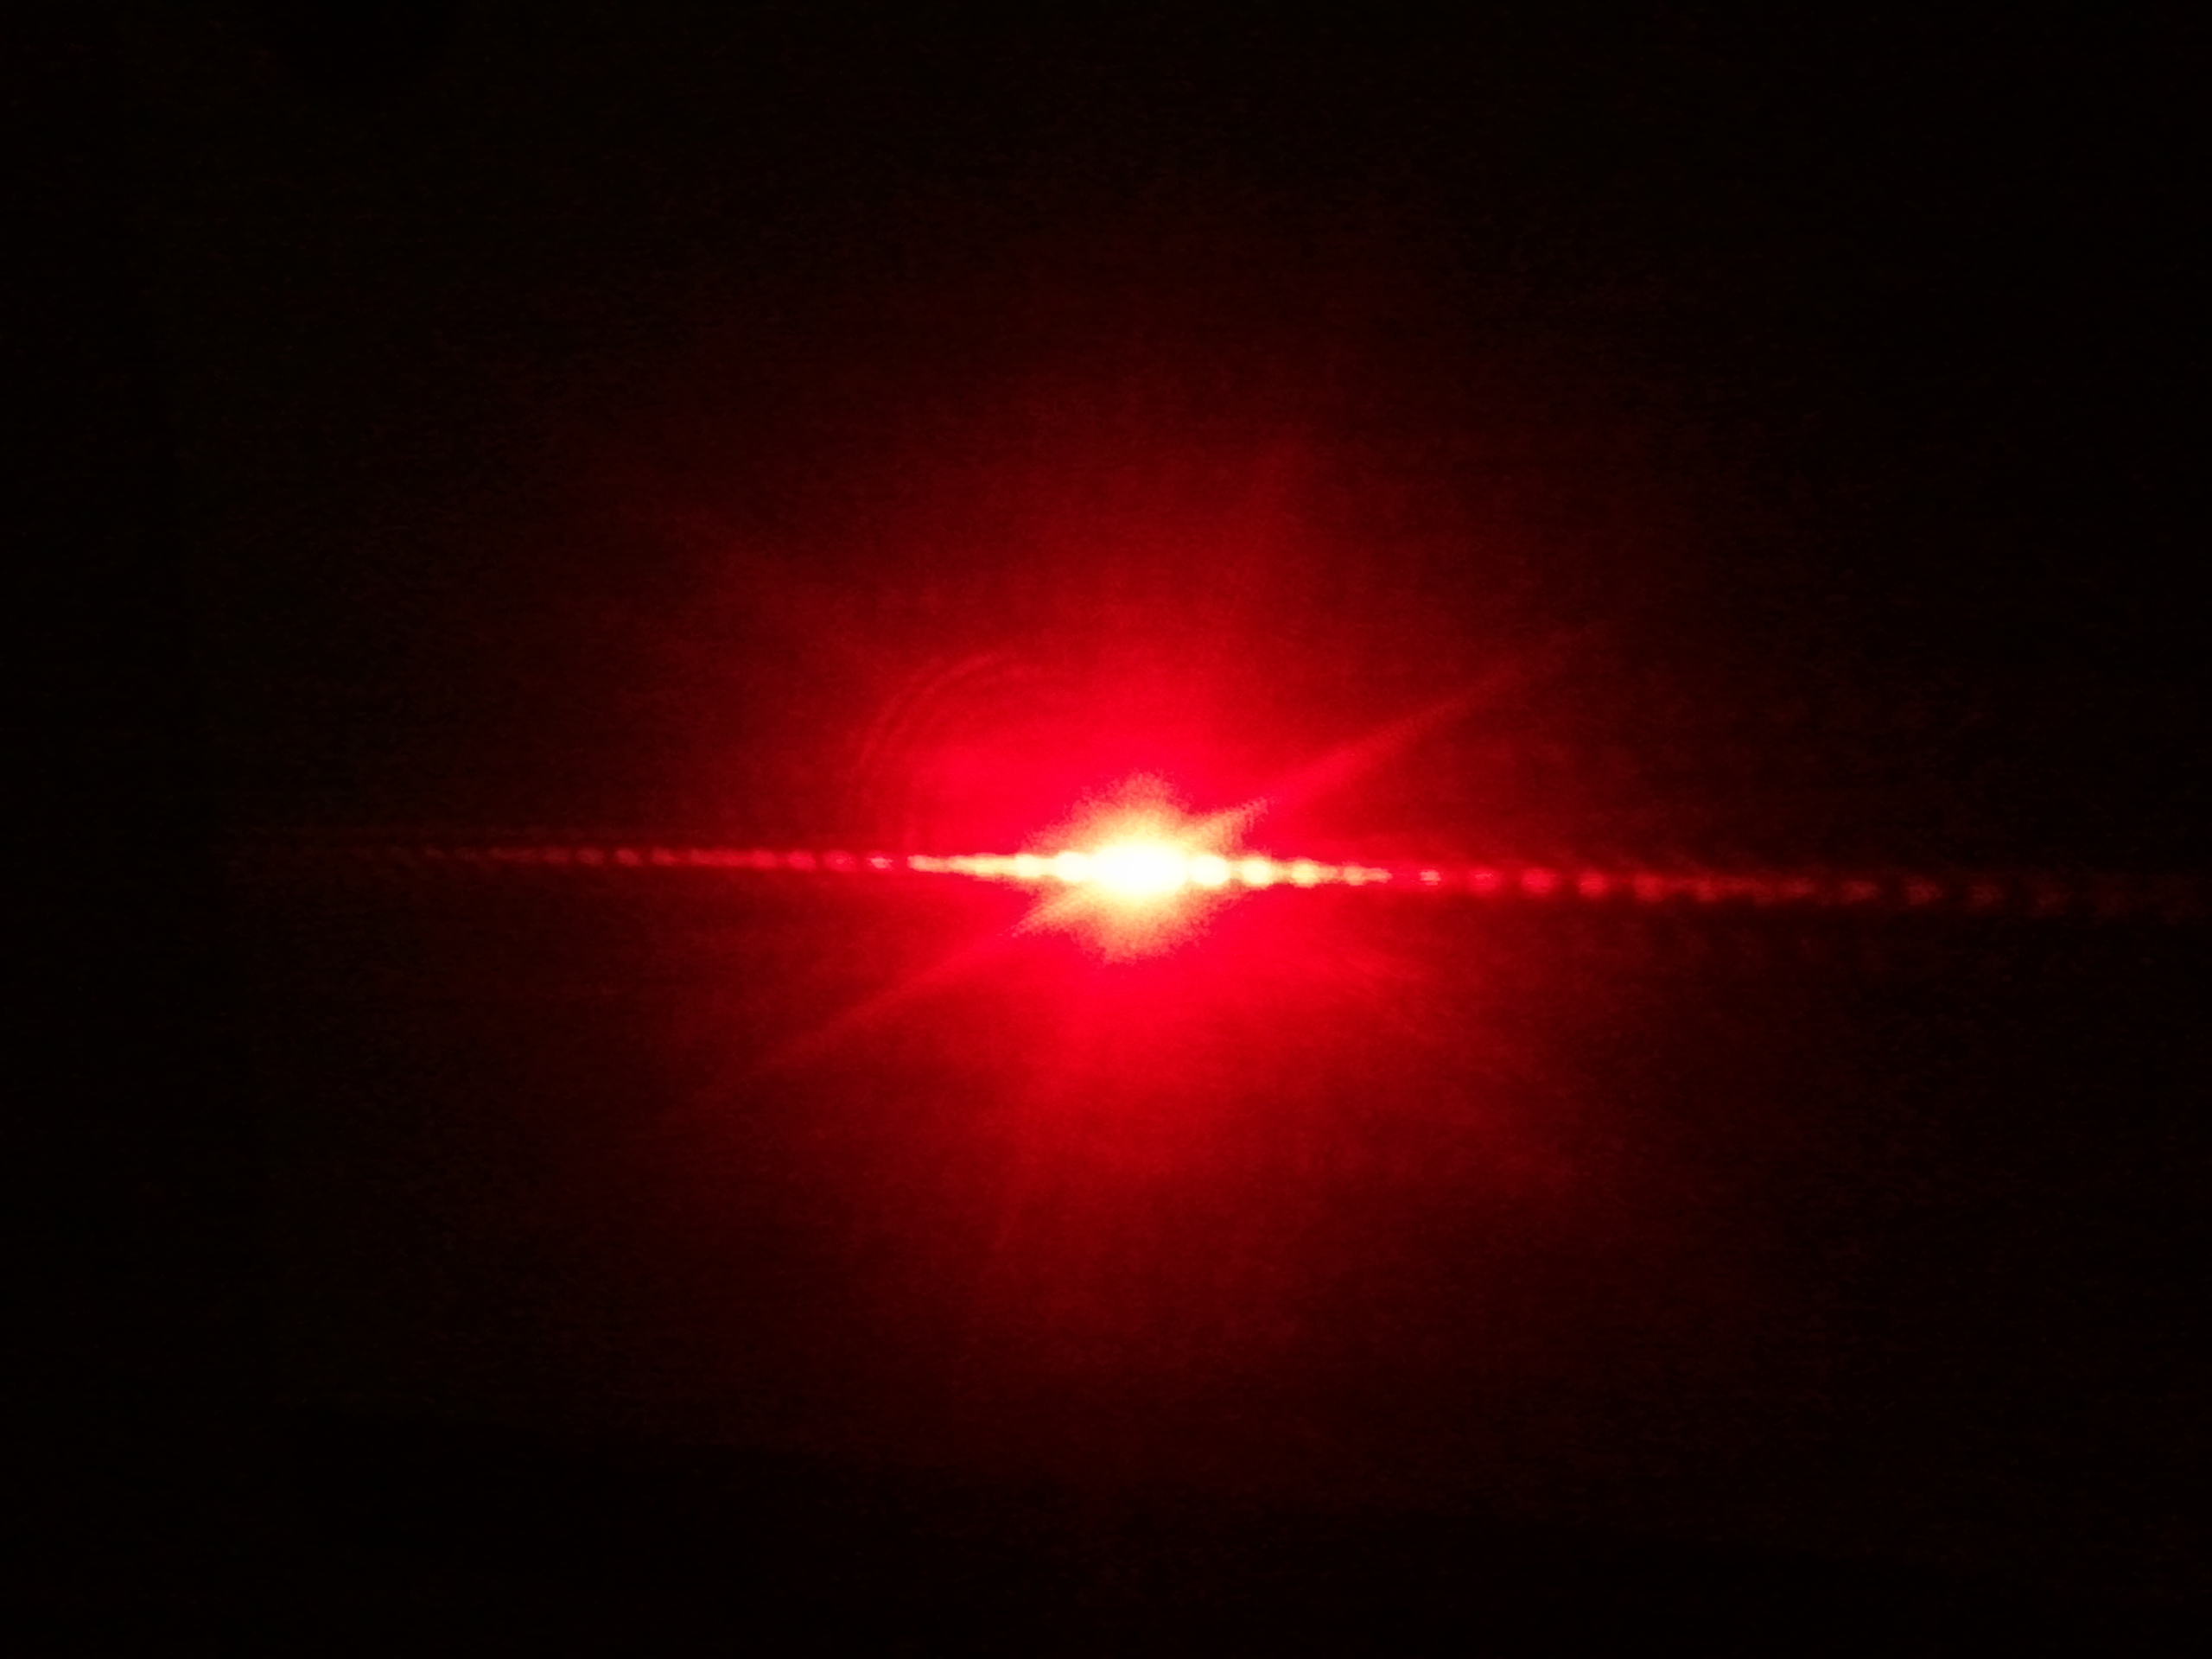
\includegraphics[width=\textwidth,natwidth=2560,natheight=1920]{Bilder/Dreifachspalt.jpg}
          \caption{Dreifachspalt}
        \end{subfigure}
\end{figure}
\subsection{Gitterkonstante eines Strichgitters}
Das Beugungsbild des Gitters wurde wieder ausgemessen. Die Werte wurden folgendermaßen aufgetragen:
\begin{align*}
y_n=\lambda l g \cdot n
\end{align*}
Hieraus kann dann die Gitterkonstante g bestimmt werden:
\begin{align*}
g=\SI{7,268}{mm^{-1}}
\end{align*}
Auch dieser Wert weicht deutlich von der Angabe ab, ist aber aufgrund der Messungenauigkeiten noch in Ordnung. Man muss bedenken, dass auch das Gitter nicht beliebig genau gearbeitet wurde.
\begin{figure}
          \centering
          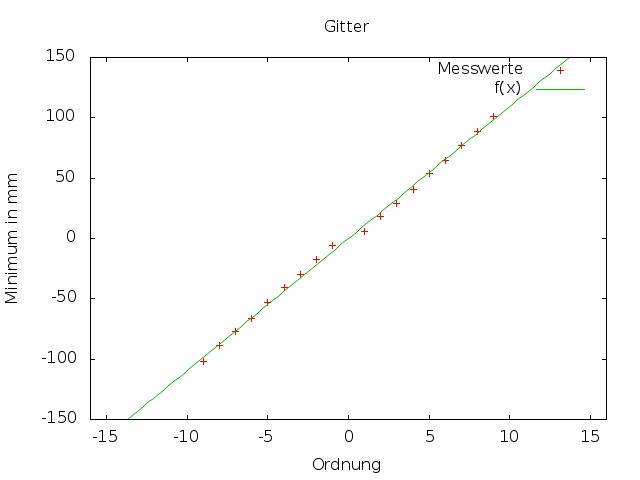
\includegraphics[width=\textwidth,natwidth=2560,natheight=1920]{Diagramme/gitter.jpg}
          \caption{Bestimmung der Gitterkonstanten}
          \end{figure}
\subsection{Beugungsbilder von Kreuz- und Wabengittern}
Bei dem Kreuzgitter sieht man die Überlagerung, wie man sie erwartet.
Auch das Beugungsbild des Wabengitters ist schön anzusehen.
\begin{figure}[!h]
\centering
        \begin{subfigure}[!h]{0.49\textwidth}
          \centering
          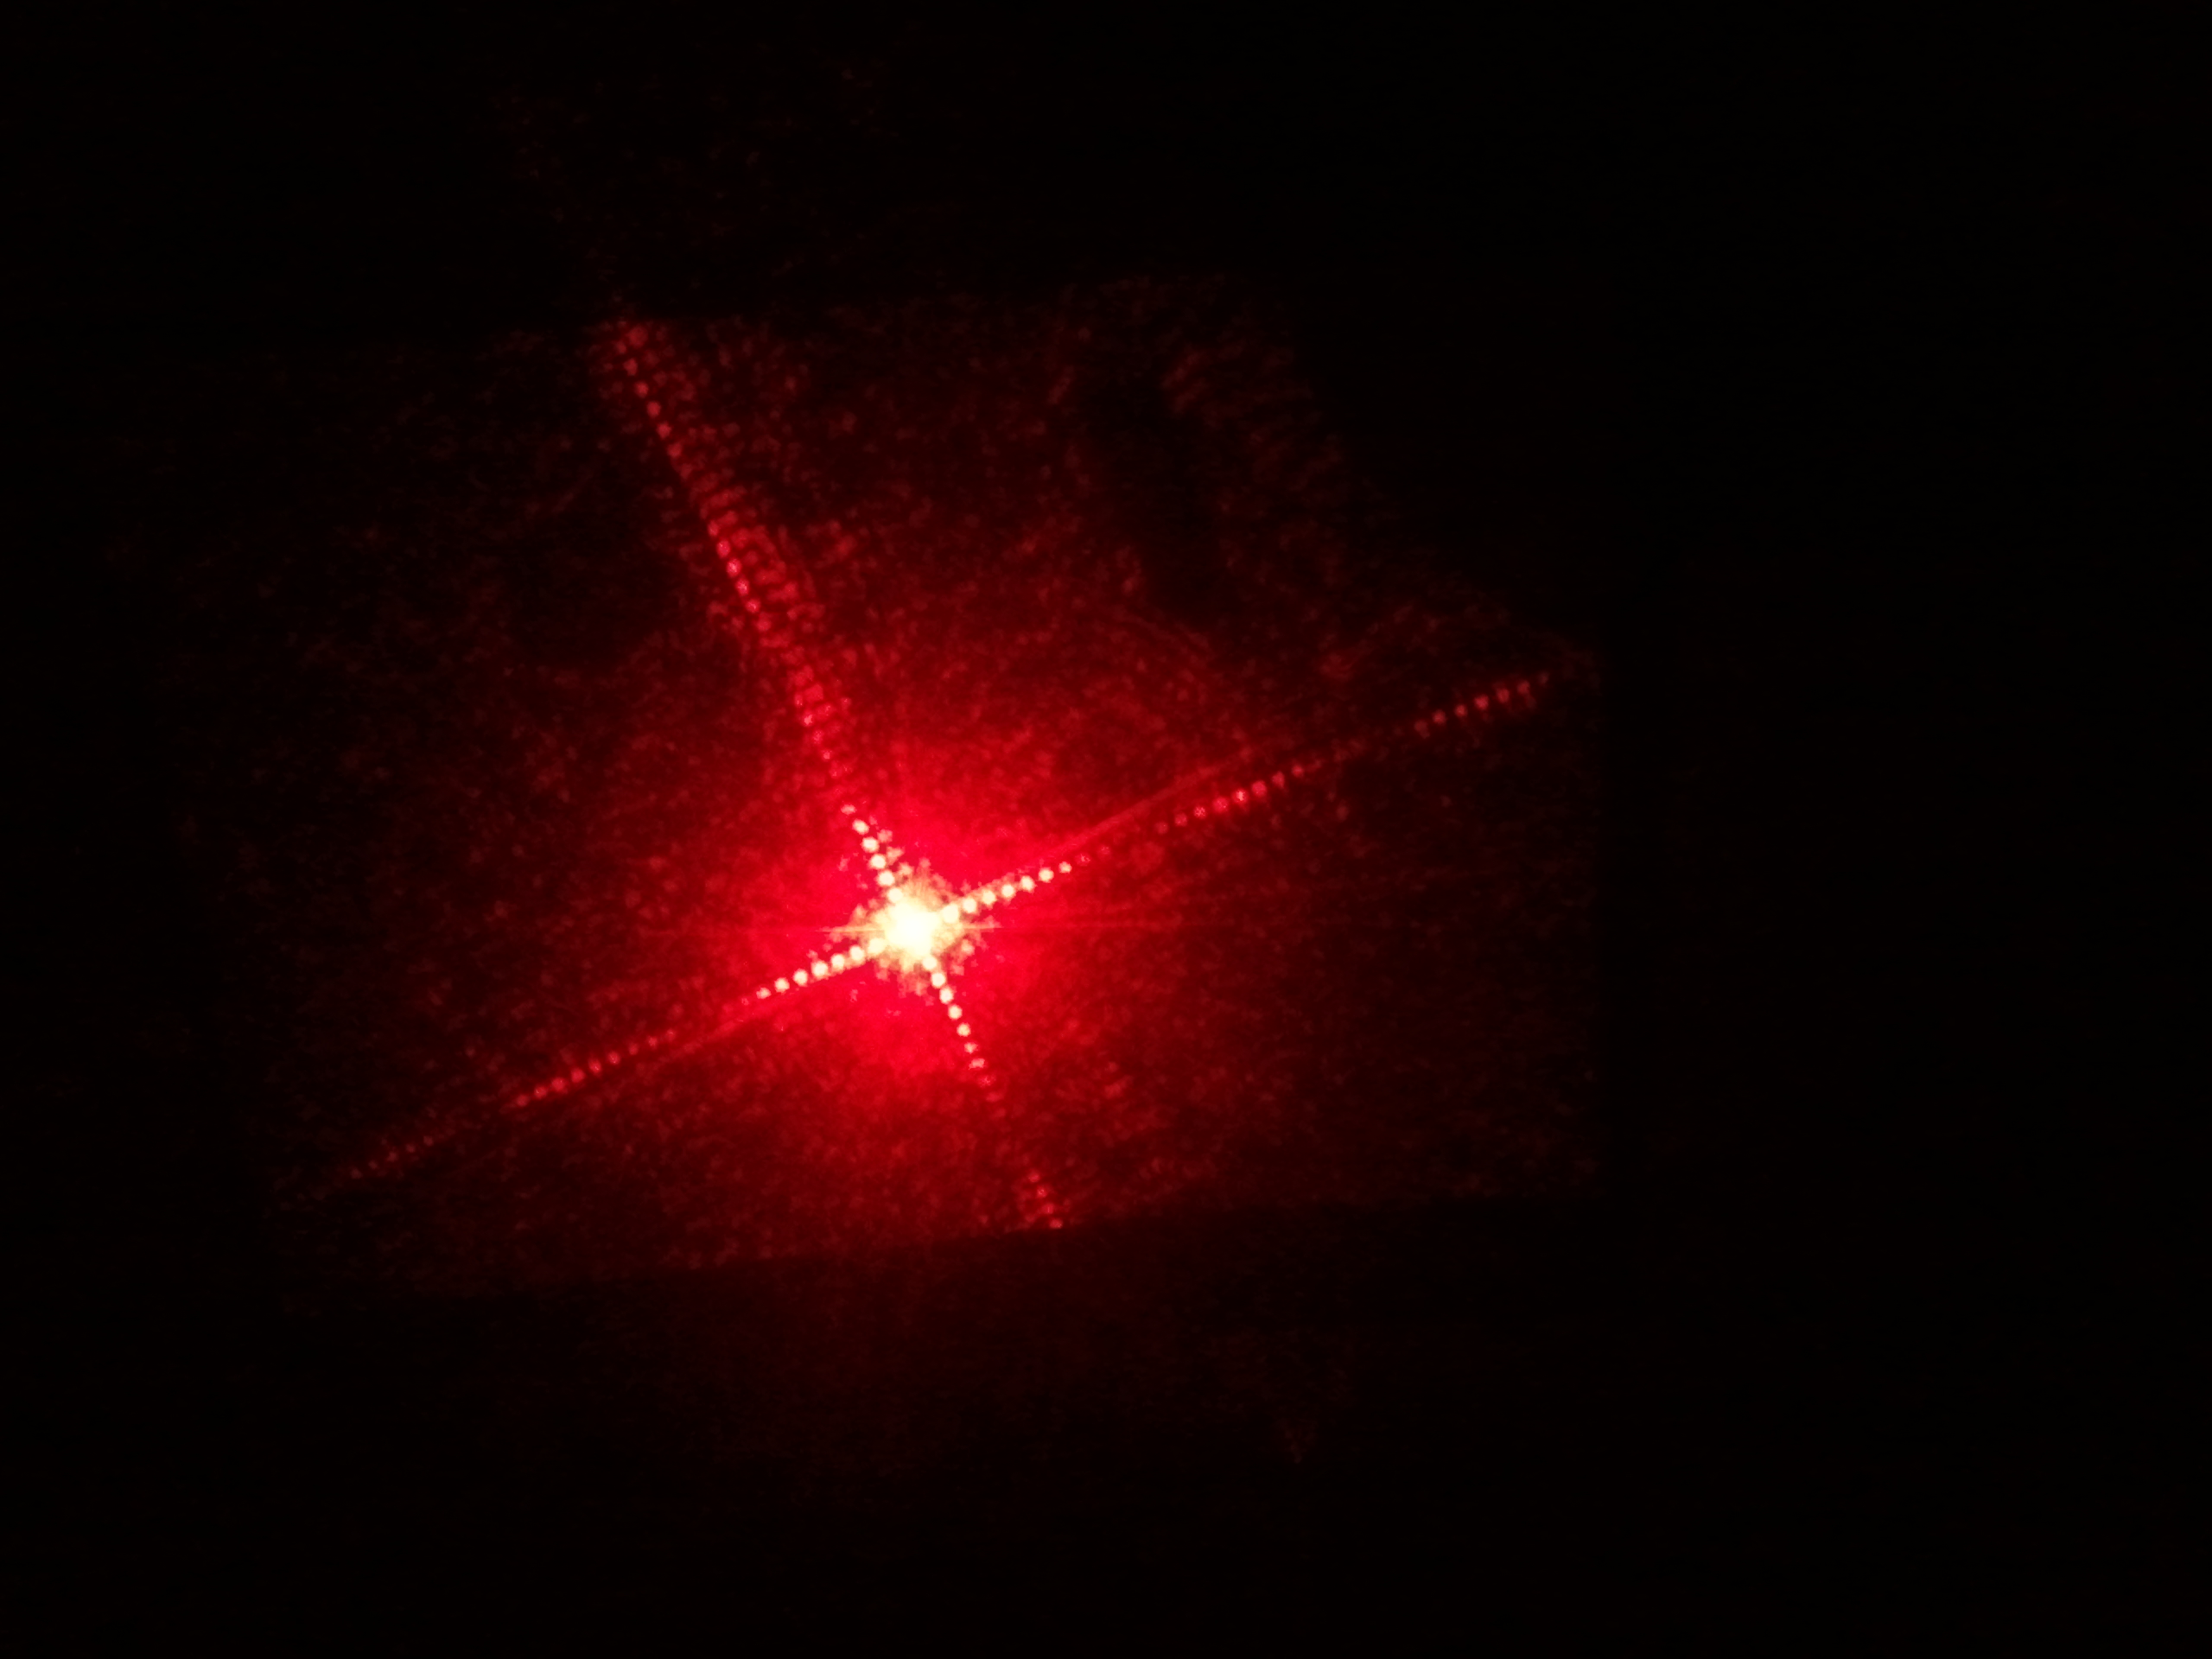
\includegraphics[width=\textwidth,natwidth=2560,natheight=1920]{Bilder/Kreuzgitter.jpg}
          \caption{Kreuzgitter}
        \end{subfigure}
        \begin{subfigure}[!h]{0.49\textwidth}
          \centering
          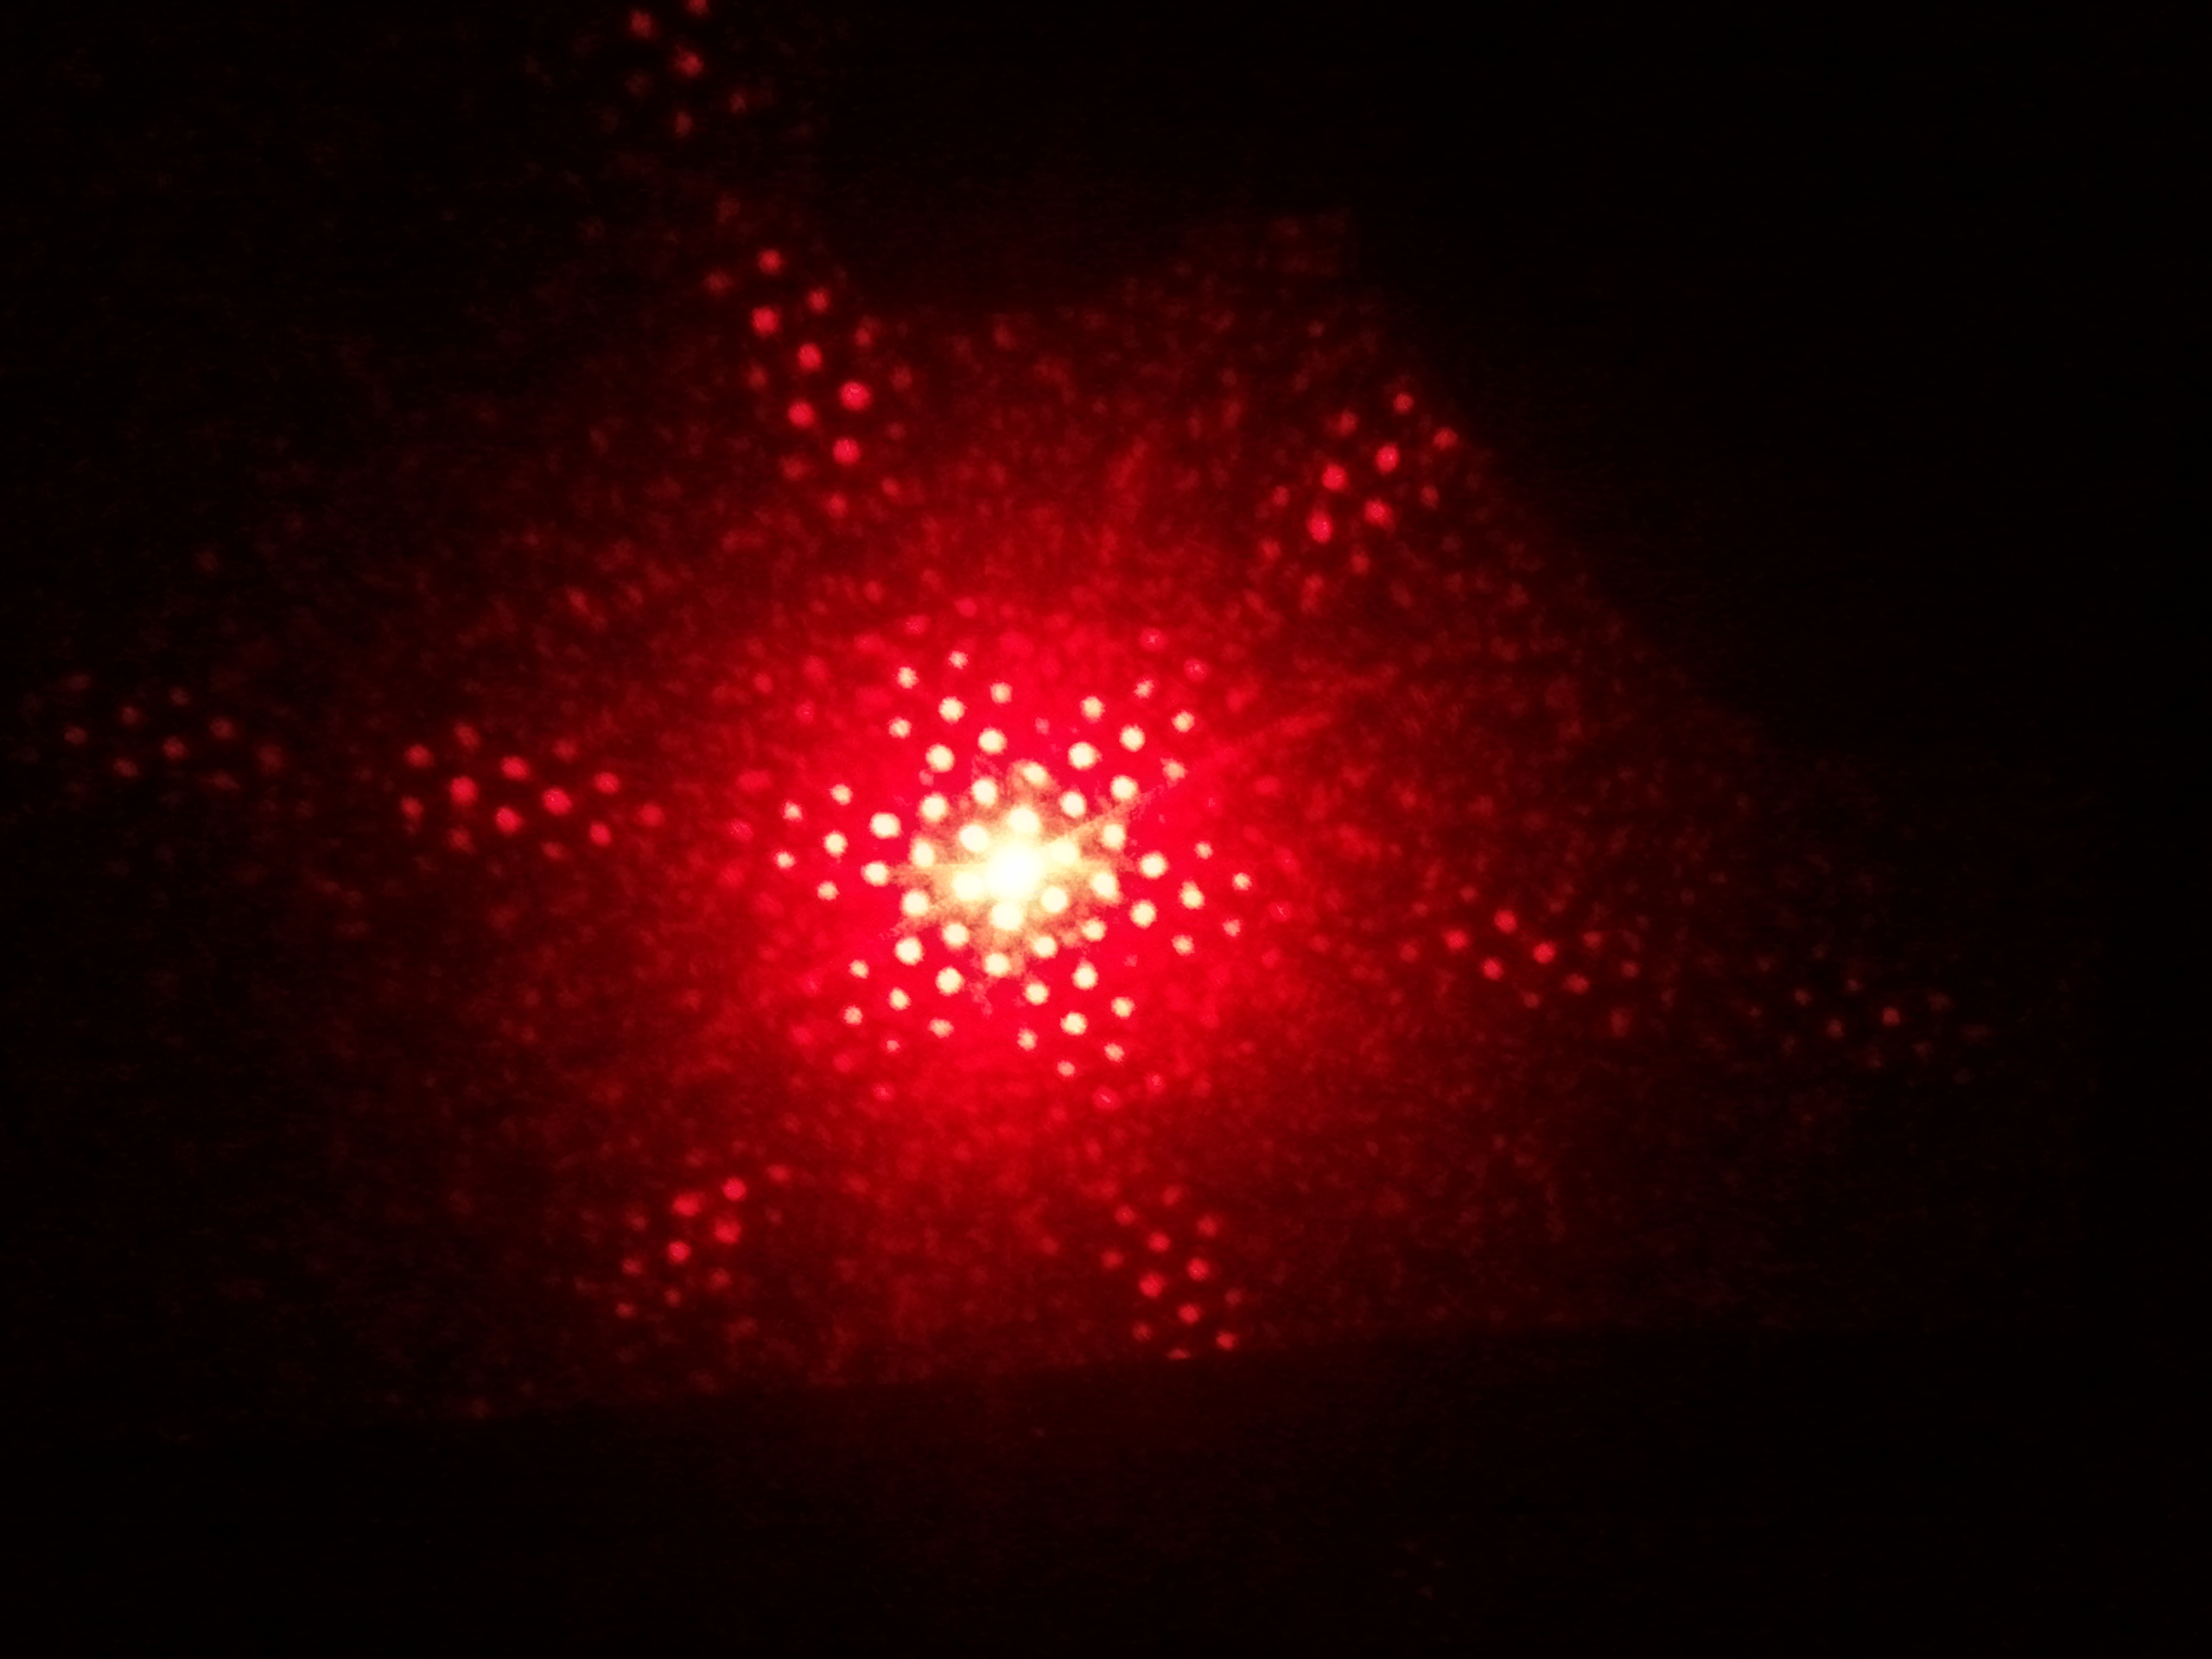
\includegraphics[width=\textwidth,natwidth=2560,natheight=1920]{Bilder/Wabengitter.jpg}
          \caption{Wabengitter}
        \end{subfigure}
\end{figure}
\section{Bedeutung der Beugungsordnungen}
Wir beobachteten, dass bei Durchlass der nullten Ordnung nur ein Fleck zu sehen war. Erst mit den zusätzlichen Ordnungen wurde die Information des Gegenstandes auf das Bild übertragen. Die erste Ordnung enthielt zwar schon Information aber erst mit zusätzlichen Ordnungen konnte das Bild scharf dargestellt werden.
\section{Holographie}
Wir beobachteten zuerst ein Hologramm, dass speziell für die Wellenlänge des Lasers hergestellt wurde. Hier bestätigt sich unsere Annahme, dass in diesem Bild nun auch die Phasenunterschiede berücksichtigt wurden, wodurch verdeckte Schriften lesbar werden, indem man den Kopf relativ zum Bild bewegt. Auch für Weißlicht war dies an einer speziellen Platte zu beobachten, diese ist aus verschiedenen Schichten für die Wellenlängen aufgebaut.



\end{document}
